\documentclass[../AnalysisNoteJBuxton.tex]{subfiles}
\begin{document}

\subsection{Residual Correlations}
\label{ResidualCorrelations}

The purpose of this analysis is study the interaction and scale of the emitting source of the pairs.
In order to obtain correct results, it is important for our particle collections to consist of primary particles.
In practice, this is difficult to achieve for our $\Lambda$ and $\bar{\Lambda}$ collections.
Many of our $\Lambda$ particles are not primary, but originate as decay products from other hyperons, including $\Sigma^{0}$, $\Xi^{0}$, $\Xi^{-}$ and $\Sigma^{*(+,-,0)}(1385)$.  Additionally, many of our K particles are not primary, but decay from K$^{*(+,-,0)}(892)$ parents.
In these decays, the $\Lambda$ carries away a momentum very similar to that of its parent.
As a result, the correlation function between a secondary $\Lambda$ and, for instance, a K$^{+}$  will be sensitive to, and dependent upon, the interaction between the parent of the $\Lambda$ and the K$^{+}$.
In effect, the correlation between the parent of the $\Lambda$ and the K$^{+}$ (ex. $\Sigma^{0}$K$^{+}$) will be visible, although smeared out, in the $\Lambda$K$^{+}$ data.
We call this a residual correlation resulting from feed-down.

As it is difficult for us to eliminate these residual correlations in our analyses, we must attempt to account for them in our fitter.
To achieve this, we will simultaneously fit the data for both the primary correlation function and the residual correlations.  For example, in the simple case of a $\Lambda$K$^{+}$ analysis with residuals arising soley from $\Sigma^{0}$K$^{+}$ feed-down:

\begin{equation}
\begin{array}{l}
\vspace{4mm}
 C_{measured}(k^{*}_{\Lambda K^{+}}) = 1 + \lambda_{\Lambda K^{+}}[C_{\Lambda K^{+}}(k^{*}_{\Lambda K^{+}})-1] + \lambda_{\Sigma^{0}K^{+}}[C_{\Sigma^{0}K^{+}}(k^{*}_{\Lambda K^{+}})-1] \\
\vspace{2mm}
  ~~~~~C_{\Sigma^{0}K^{+}}(k^{*}_{\Lambda K^{+}}) \equiv \frac{\sum\limits_{k^{*}_{\Sigma^{0}K^{+}}} C_{\Sigma^{0}K^{+}}\left(k^{*}_{\Sigma^{0}K^{+}}\right) T\left(k^{*}_{\Sigma^{0}K^{+}},k^{*}_{\Lambda K^{+}}\right)}{\sum\limits_{k^{*}_{\Sigma^{0}K^{+}}} T\left(k^{*}_{\Sigma^{0}K^{+}},k^{*}_{\Lambda K^{+}}\right)}
\end{array} 
\label{eqn:SimpleResiduals}
\end{equation}

$C_{\Sigma^{0}K^{+}}(k^{*}_{\Sigma^{0}K^{+}})$ is the $\Sigma^{0}$K$^{+}$ correlation function from, for instance, Equation \ref{eqn:LednickyEqn}, and $T$ is the transform matrix generated with THERMINATOR.

  This equation can be easily extended to include feed-down from more sources:

\begin{equation}
\begin{array}{l}
\vspace{4mm}
\begin{split}
 C_{measured}(k^{*}_{\Lambda K}) & = 1 + \lambda_{\Lambda K}[C_{\Lambda K}(k^{*}_{\Lambda K})-1] + \lambda_{\Sigma^{0}K}[C_{\Sigma^{0}K}(k^{*}_{\Lambda K})-1] + ... \\ &
 + \lambda_{P_{1}P_{2}}[C_{P_{1}P_{2}}(k^{*}_{\Lambda K})-1] + \lambda_{other}[C_{other}(k^{*}_{\Lambda K})-1] 
\end{split}
\\
\vspace{2mm}
  ~~~~~C_{P_{1}P_{2}}(k^{*}_{\Lambda K}) \equiv \frac{\sum\limits_{k^{*}_{P_{1}P_{2}}} C_{P_{1}P_{2}}\left(k^{*}_{P_{1}P_{2}}\right) T\left(k^{*}_{P_{1}P_{2}},k^{*}_{\Lambda K}\right)}{\sum\limits_{k^{*}_{P_{1}P_{2}}} T\left(k^{*}_{P_{1}P_{2}},k^{*}_{\Lambda K}\right)}
\end{array} 
\label{eqn:ResidualsFull}
\end{equation}

  Or, more compactly:

\begin{equation}
 C_{measured}(k^{*}_{\Lambda K}) = 1 + \sum\limits_{i}  \lambda_{i}[C_{i}(k^{*}_{\Lambda K})-1]
\label{eqn:Residuals}
\end{equation}

The framework for extracting the necessary transform matrices from the THERMINATOR data is already in place, and has been used to generate the examples from $\Lambda$K$^{+}$ and $\bar{\Lambda}$K$^{+}$ analyses shown in Figures \ref{fig:TransformMatricesLamKchP} and \ref{fig:TransformMatricesALamKchP}.  However, these residual correlations have not yet been implemented in the fitter.

There is an obvious added complication here, as, for instance, the $\Xi^{-}$K$^{\pm}$ residuals necessitate the inclusion of the CoulombFitter into the process.  The complication of combining the two fitters is not as troubling as the increase in fitting time that this is sure to bring.  We have two solutions to bypass such a large increase in run time.  First, we can use our experimental $\Xi^{\mathrm{ch}}$K$^{\mathrm{ch}}$ data to represent all charged parent pair system.  Alternatively, we can assume the strong interaction is negligible in the charged residual, and generate the parent correlation function given radius and $\lambda$ parameters.  We find in our $\Xi^{\mathrm{ch}}$K$^{\mathrm{ch}}$ that a Coulomb-only description of the system describes, reasonable well, the broad features of the correlation.  The strong interaction is necessary for the fine details.  However, as these correlations are run through a transform matrix, which largely flattens out and fine details, a Coulomb-only description should be sufficient.

\begin{figure}[h!]
  \centering
  %%----start of first subfigure---  
  \subfloat[Transform matrix for $\Sigma$K$^{+}$ pairs into $\Lambda$K$^{+}$]{
    \label{fig:TransformMatricesLamKchP:a}
    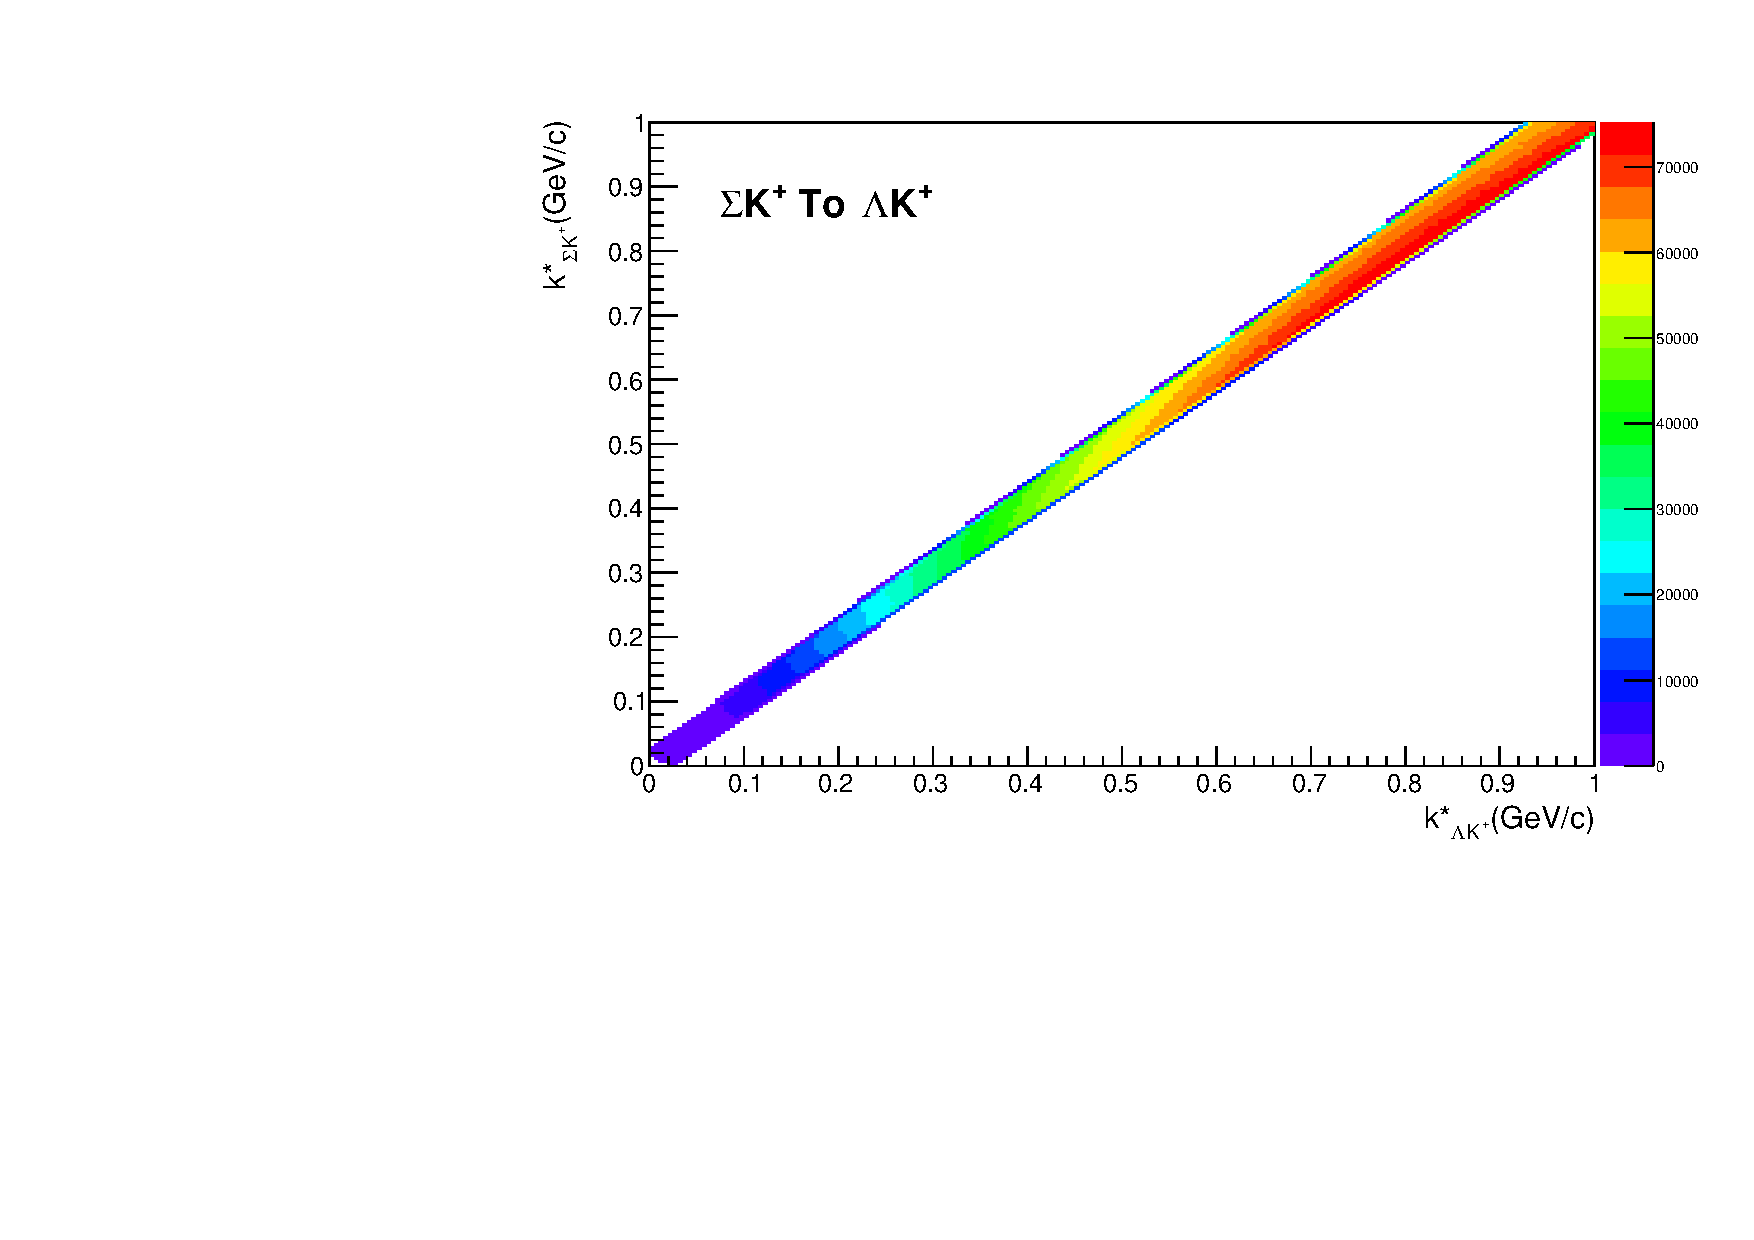
\includegraphics[width=0.49\textwidth]{5_Fitting/Figures/fSigToLamKchPTransform.pdf}}%\\
  %%----start of second subfigure---
  \subfloat[Transform matrix for $\Xi^{-}$K$^{+}$ pairs into $\Lambda$K$^{+}$]{
    \label{fig:TransformMatricesLamKchP:b}
    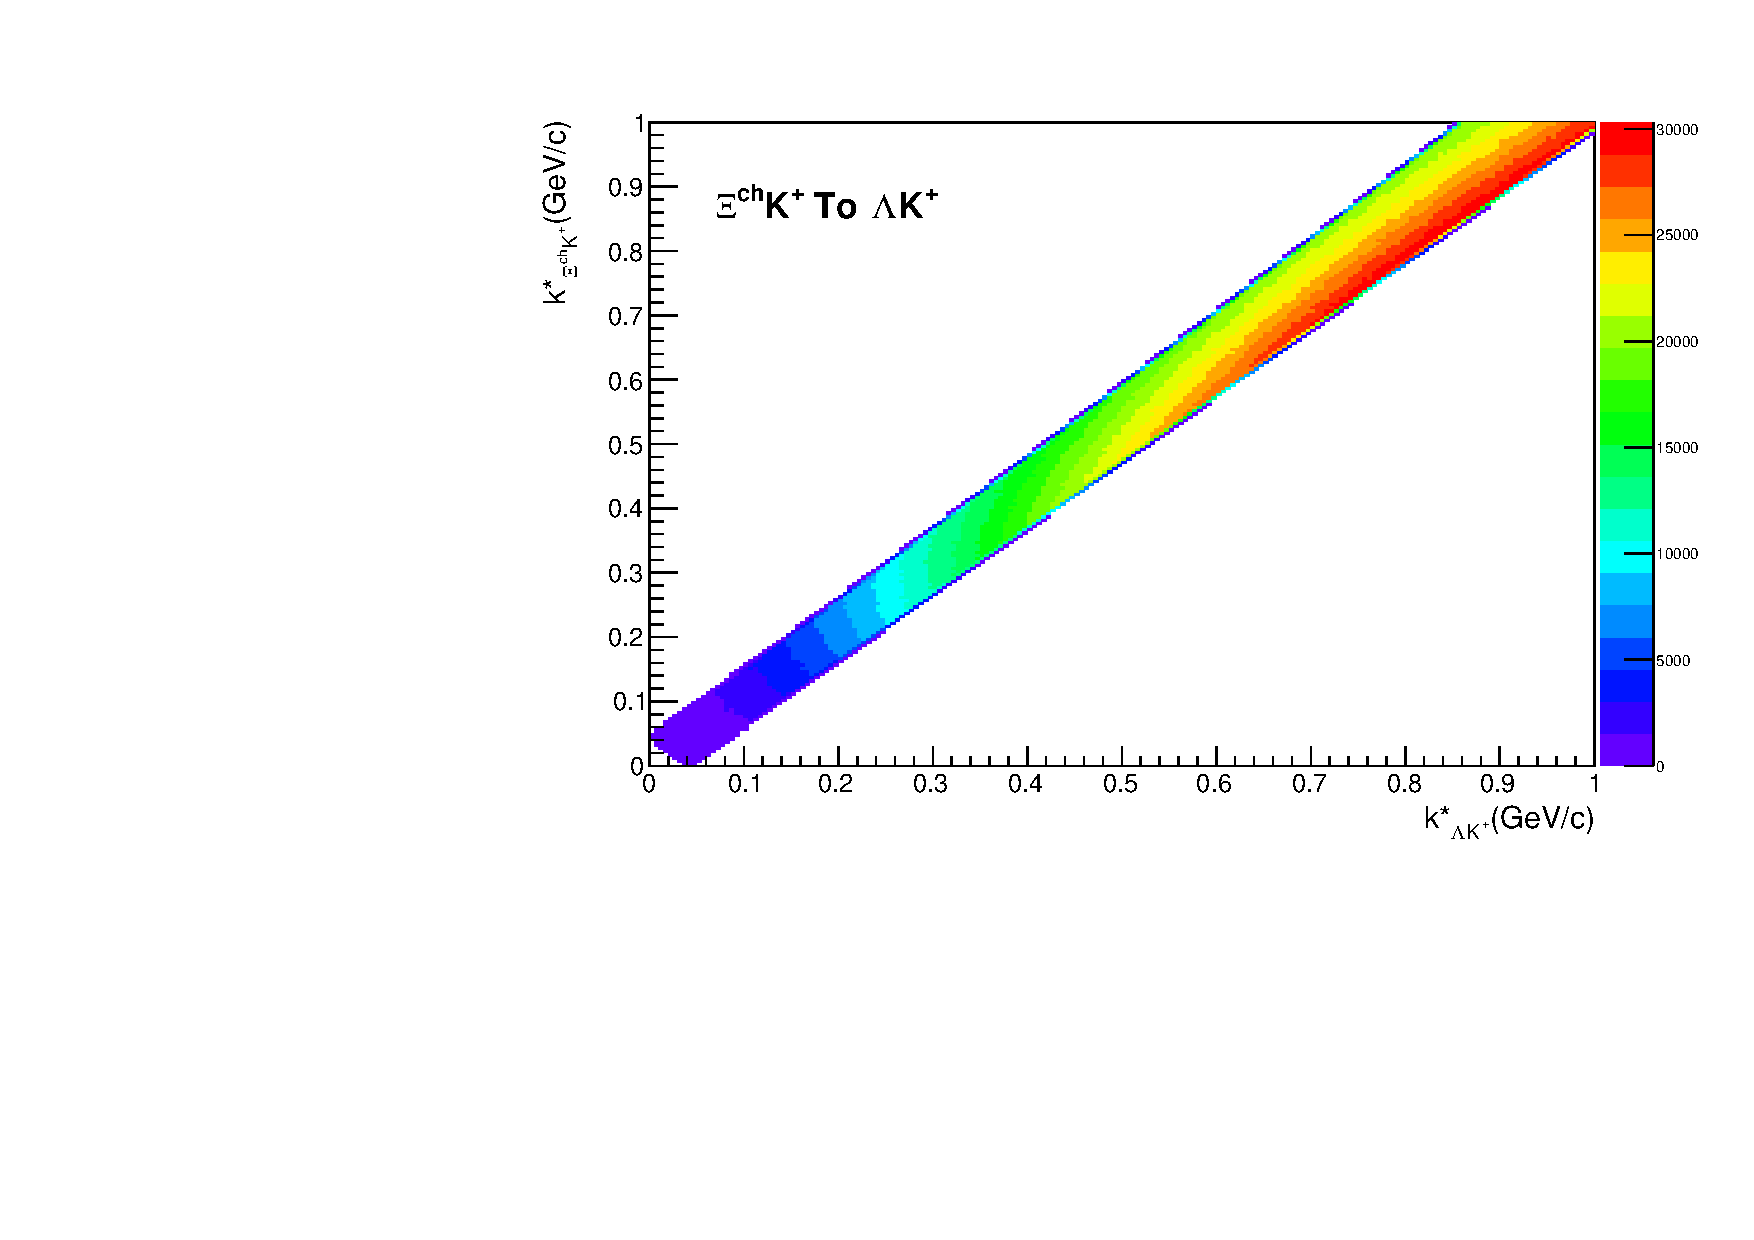
\includegraphics[width=0.49\textwidth]{5_Fitting/Figures/fXiCToLamKchPTransform.pdf}} \\
  %%----start of third subfigure---
  \subfloat[Transform matrix for $\Xi^{0}$K$^{+}$ pairs into $\Lambda$K$^{+}$]{
    \label{fig:TransformMatricesLamKchP:c}
    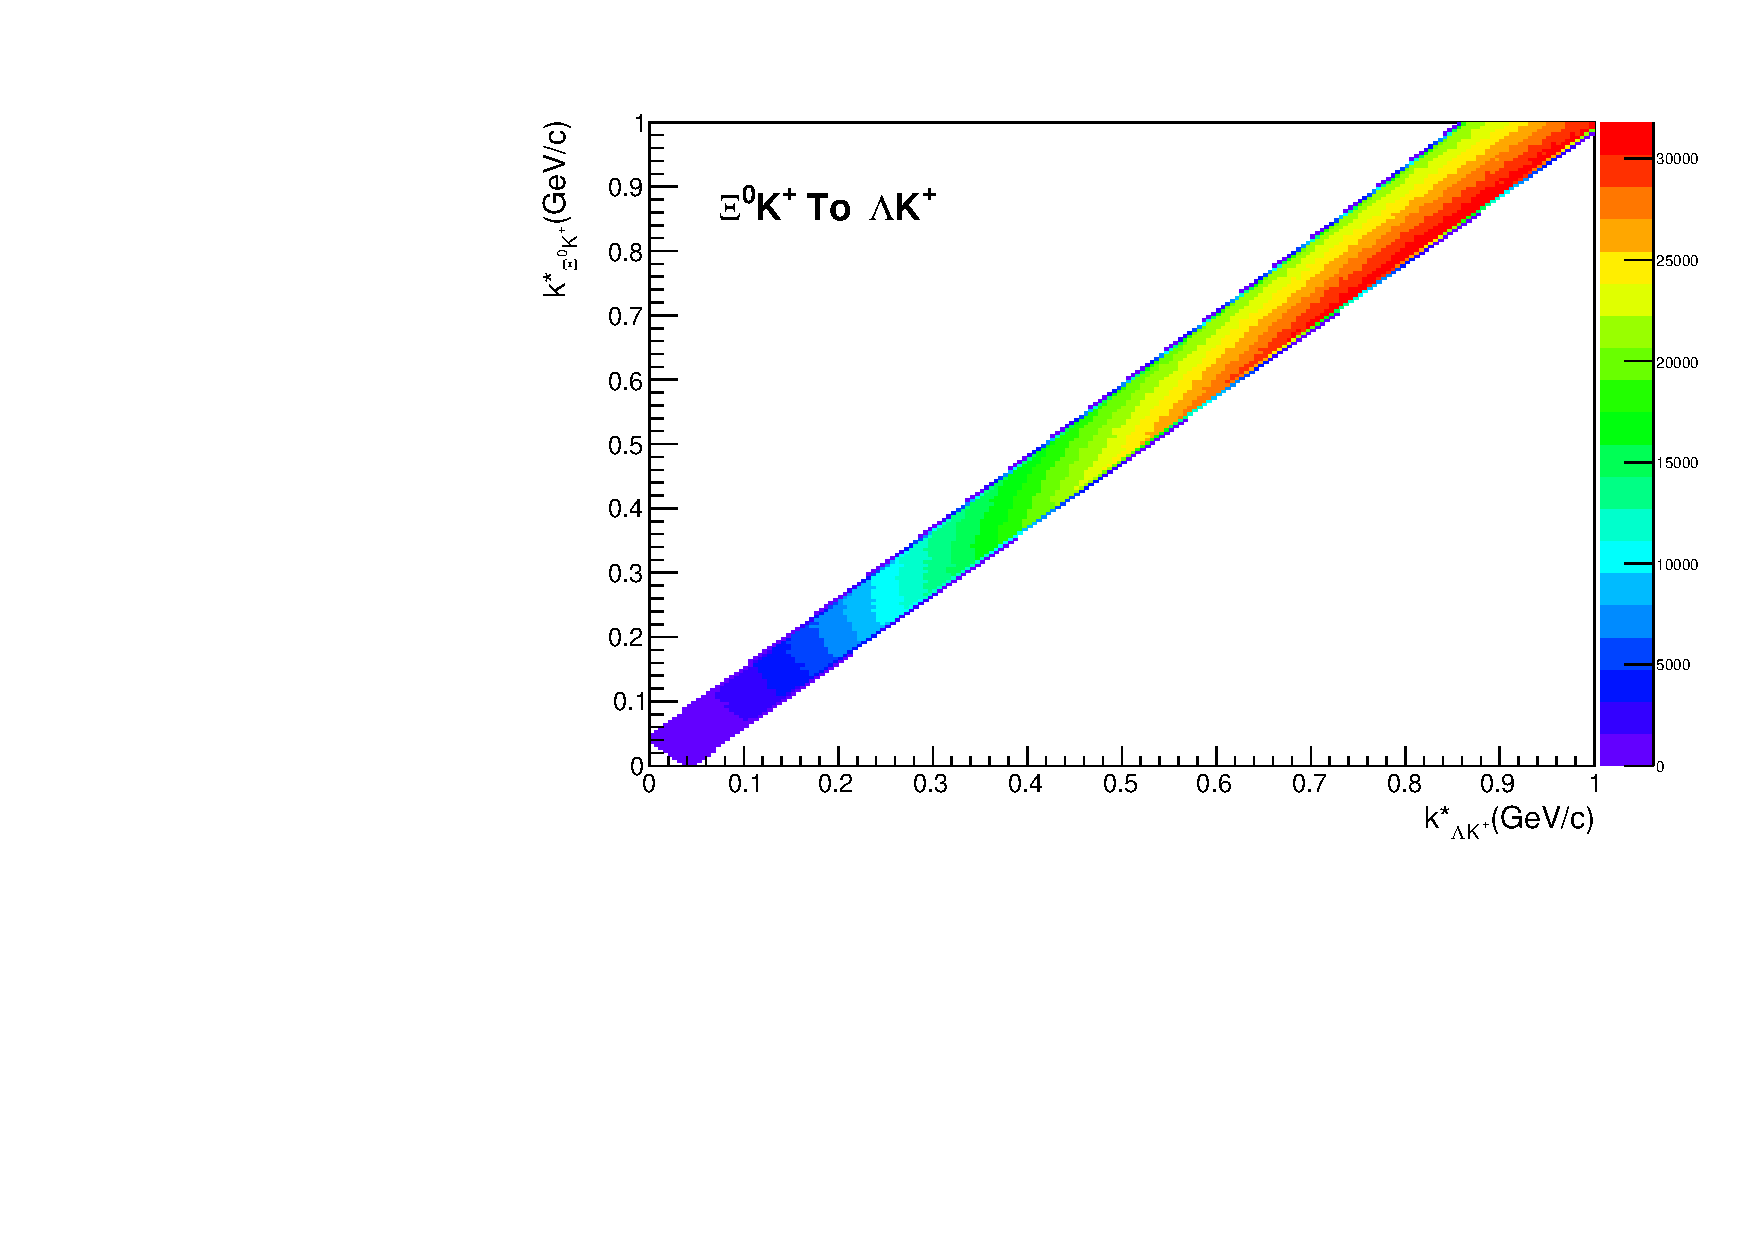
\includegraphics[width=0.49\textwidth]{5_Fitting/Figures/fXi0ToLamKchPTransform.pdf}}
  %%----start of fourth subfigure---
  \subfloat[Transform matrix for $\Omega^{-}$K$^{+}$ pairs into $\Lambda$K$^{+}$]{
    \label{fig:TransformMatricesLamKchP:d}
    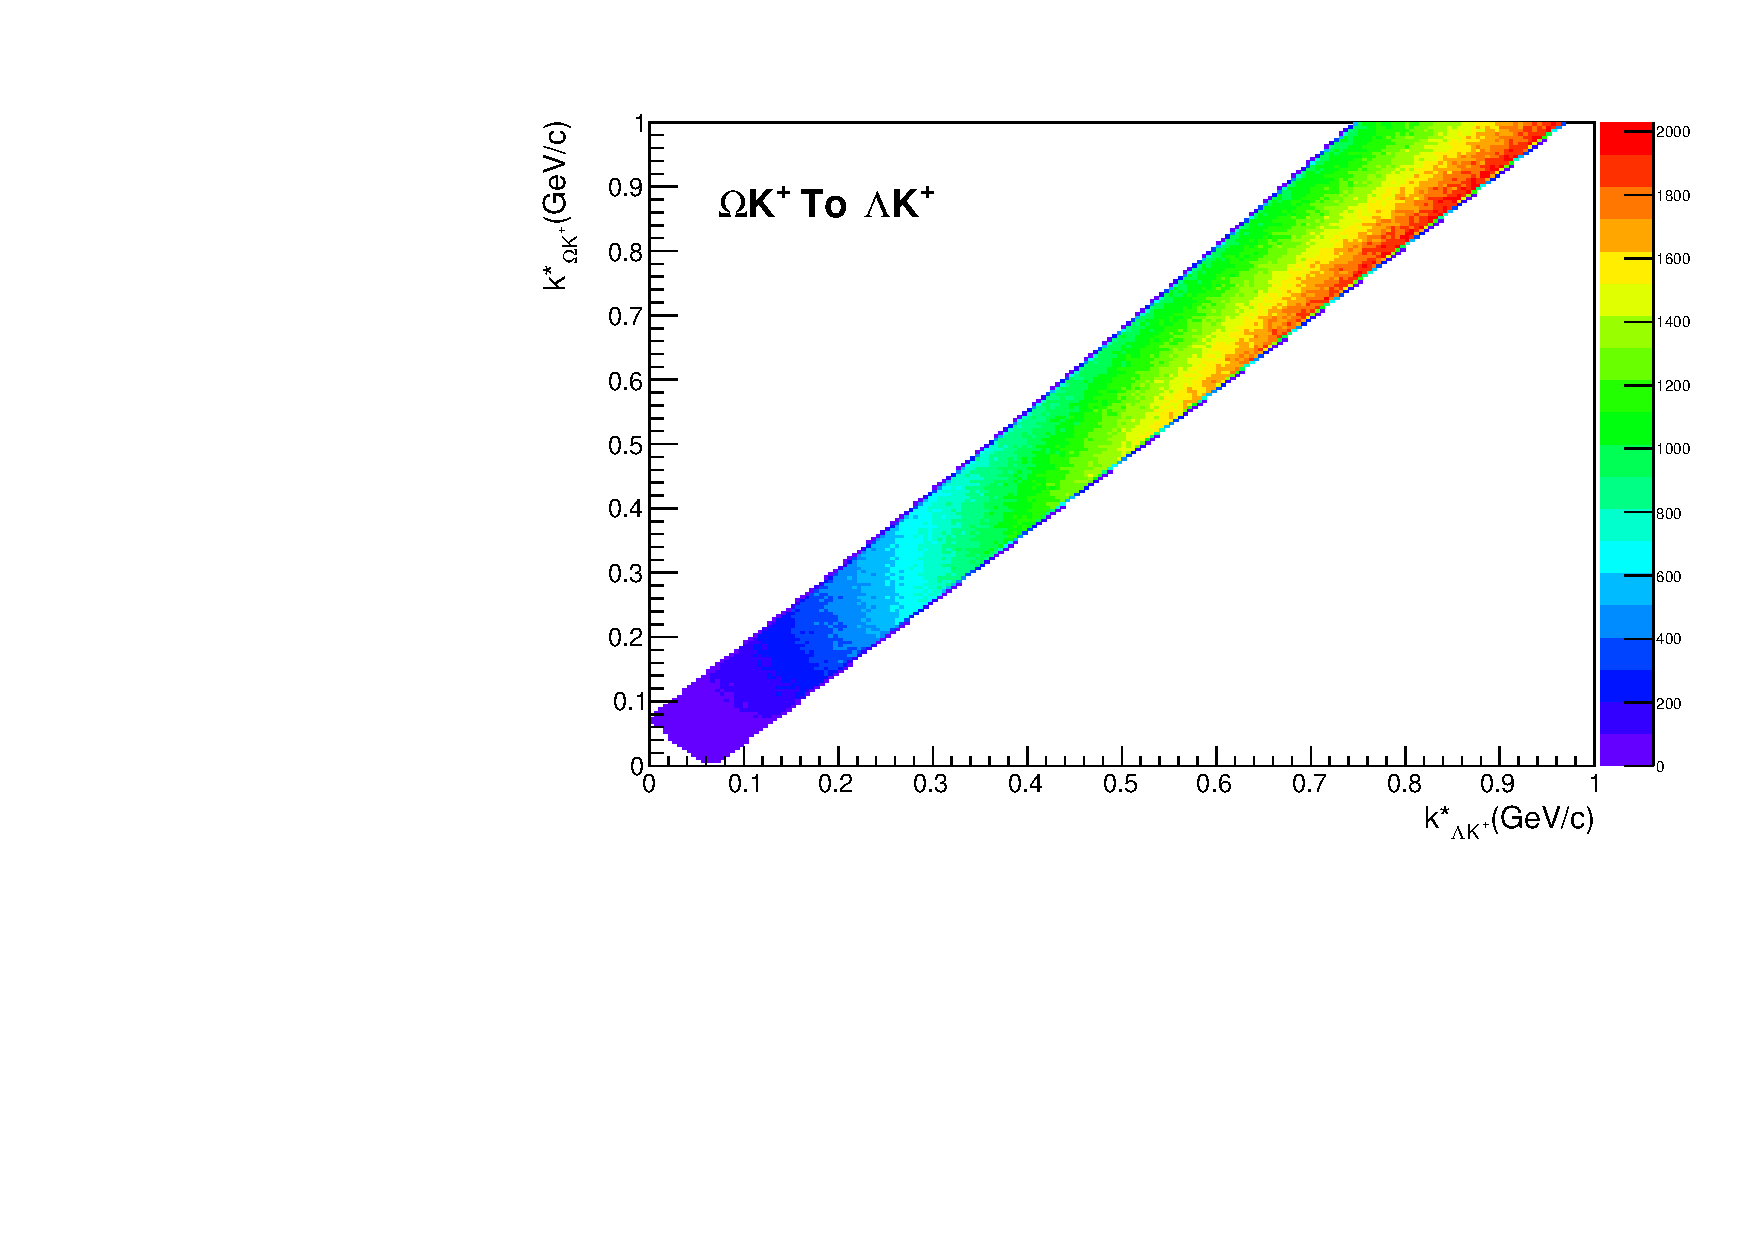
\includegraphics[width=0.49\textwidth]{5_Fitting/Figures/fOmegaToLamKchPTransform.pdf}} \\                   
  %%----overall caption----
  \caption[Transform Matrices for $\Lambda$K$^{+}$ Analysis]{Transform Matrices generated with THERMINATOR for $\Lambda$K$^{+}$ Analysis}
  \label{fig:TransformMatricesLamKchP}
\end{figure}


\begin{figure}[h!]
  \centering
  %%----start of first subfigure---
  \subfloat[Transform matrix for $\bar{\Sigma}$K$^{+}$ pairs into $\bar{\Lambda}$K$^{+}$]{
    \label{fig:TransformMatricesALamKchP:a}
    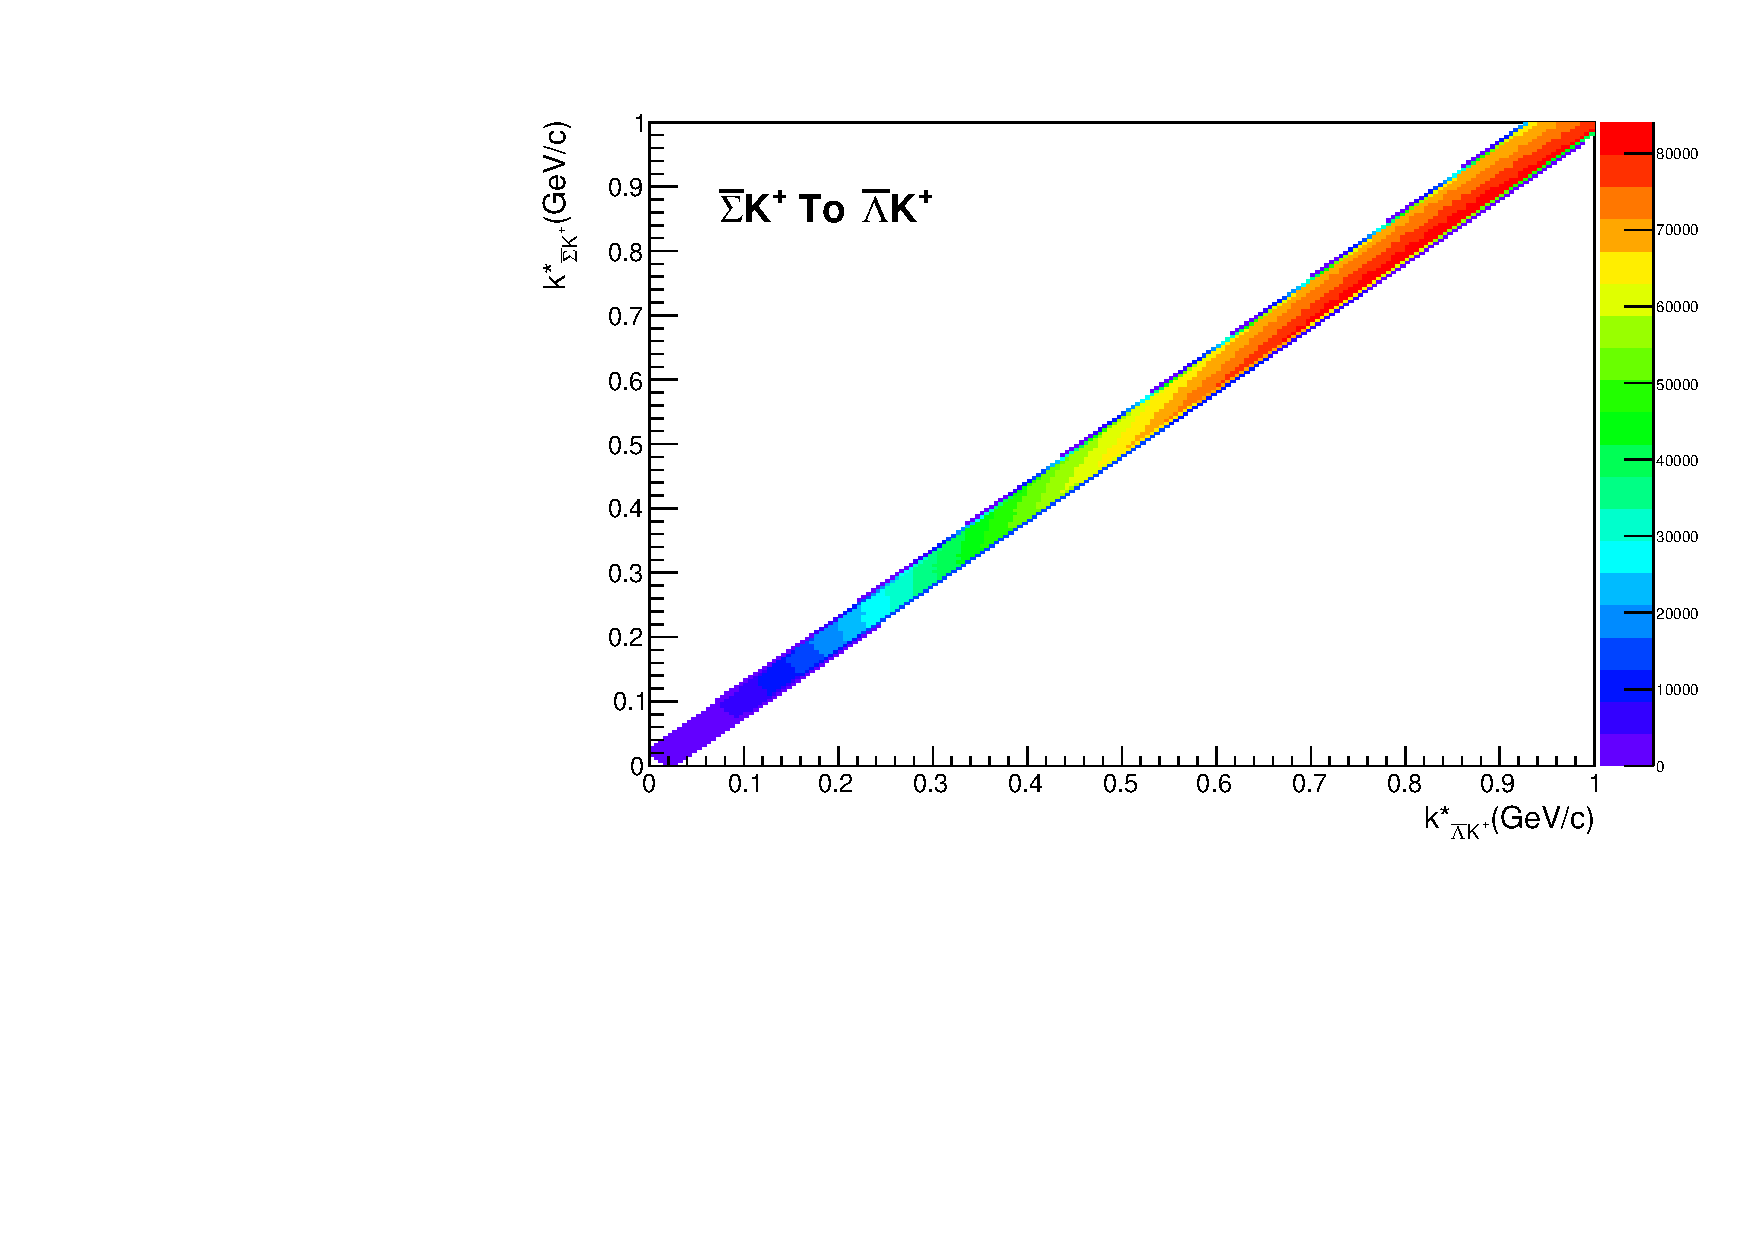
\includegraphics[width=0.49\textwidth]{5_Fitting/Figures/fASigToALamKchPTransform.pdf}}
  %%----start of second subfigure---
  \subfloat[Transform matrix for $\bar{\Xi}^{+}$K$^{+}$ pairs into $\bar{\Lambda}$K$^{+}$]{
    \label{fig:TransformMatricesALamKchP:b}
    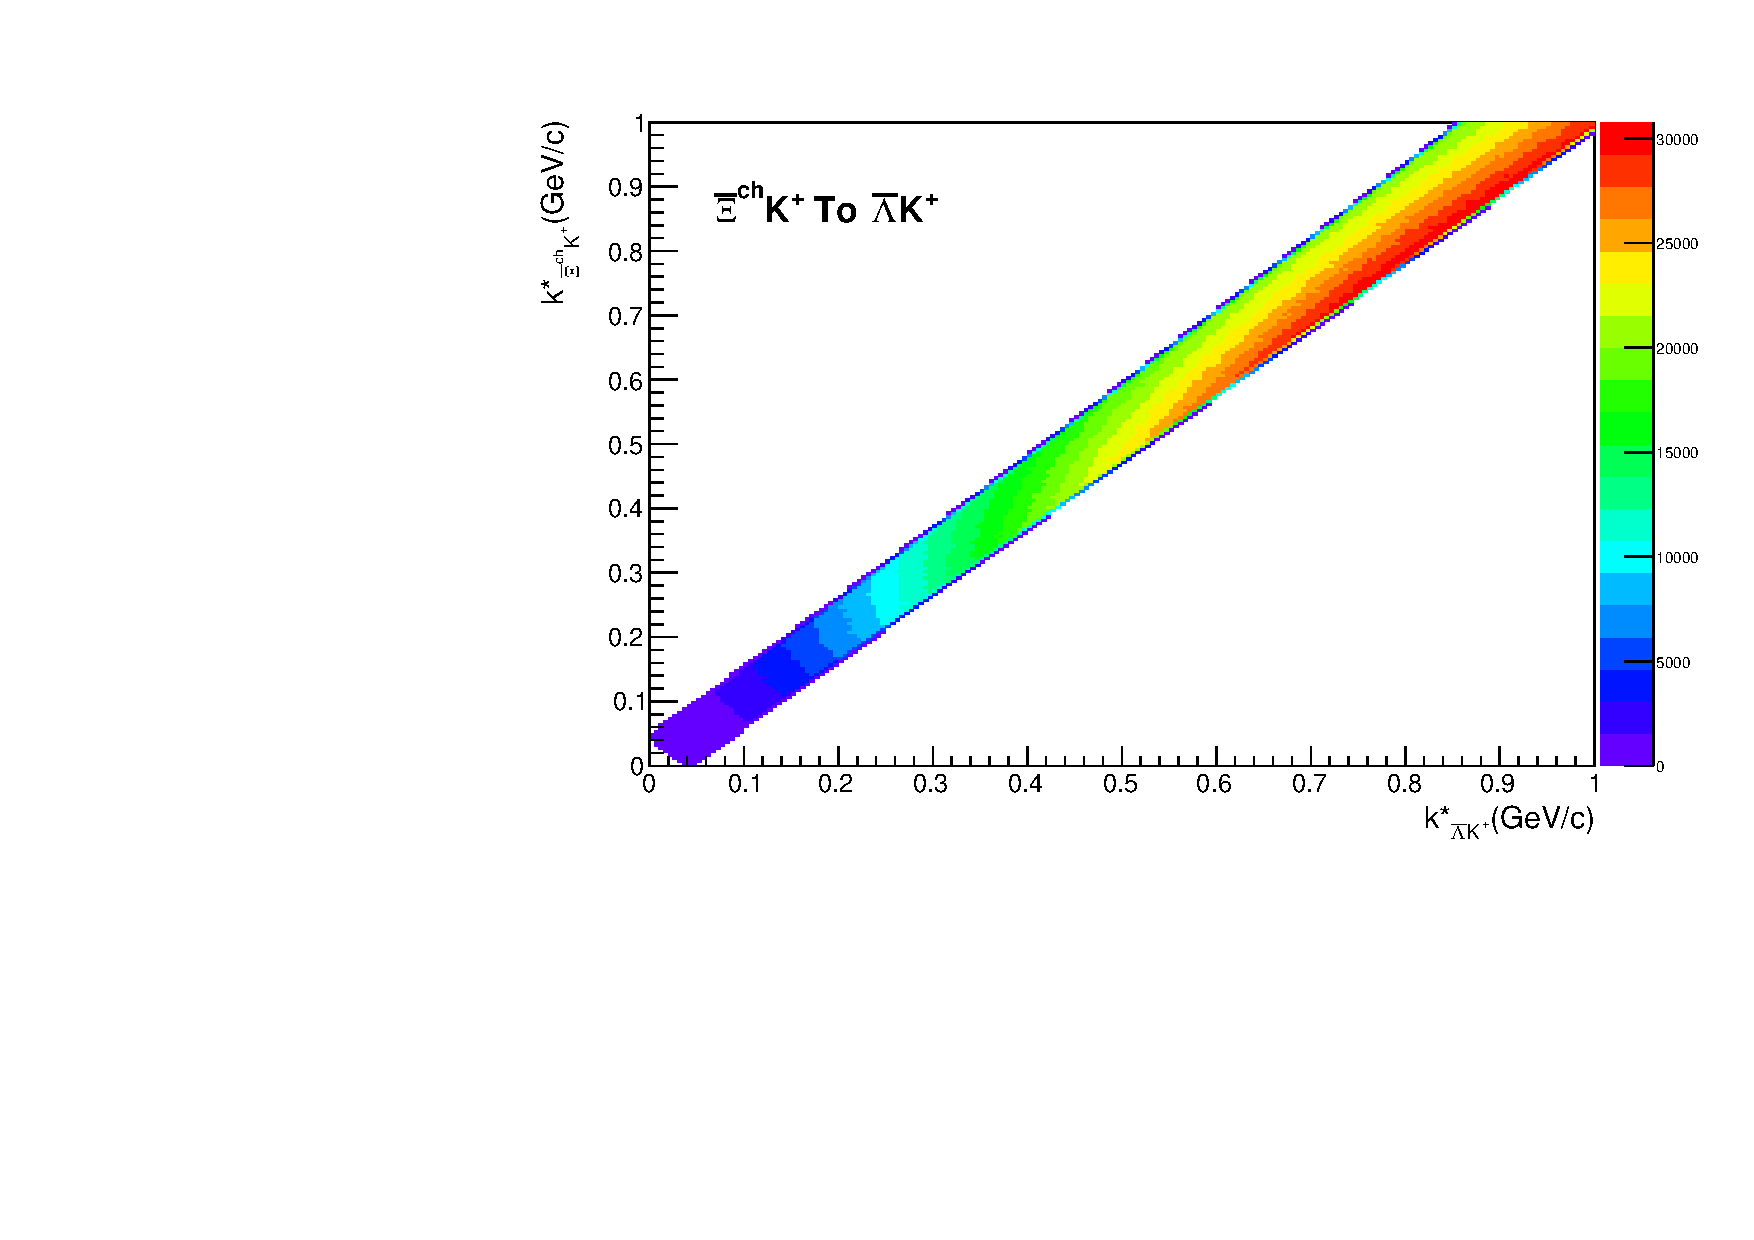
\includegraphics[width=0.49\textwidth]{5_Fitting/Figures/fAXiCToALamKchPTransform.pdf}} \\
  %%----start of third subfigure---
  \subfloat[Transform matrix for $\bar{\Xi}^{0}$K$^{+}$ pairs into $\bar{\Lambda}$K$^{+}$]{
    \label{fig:TransformMatricesALamKchP:c}
    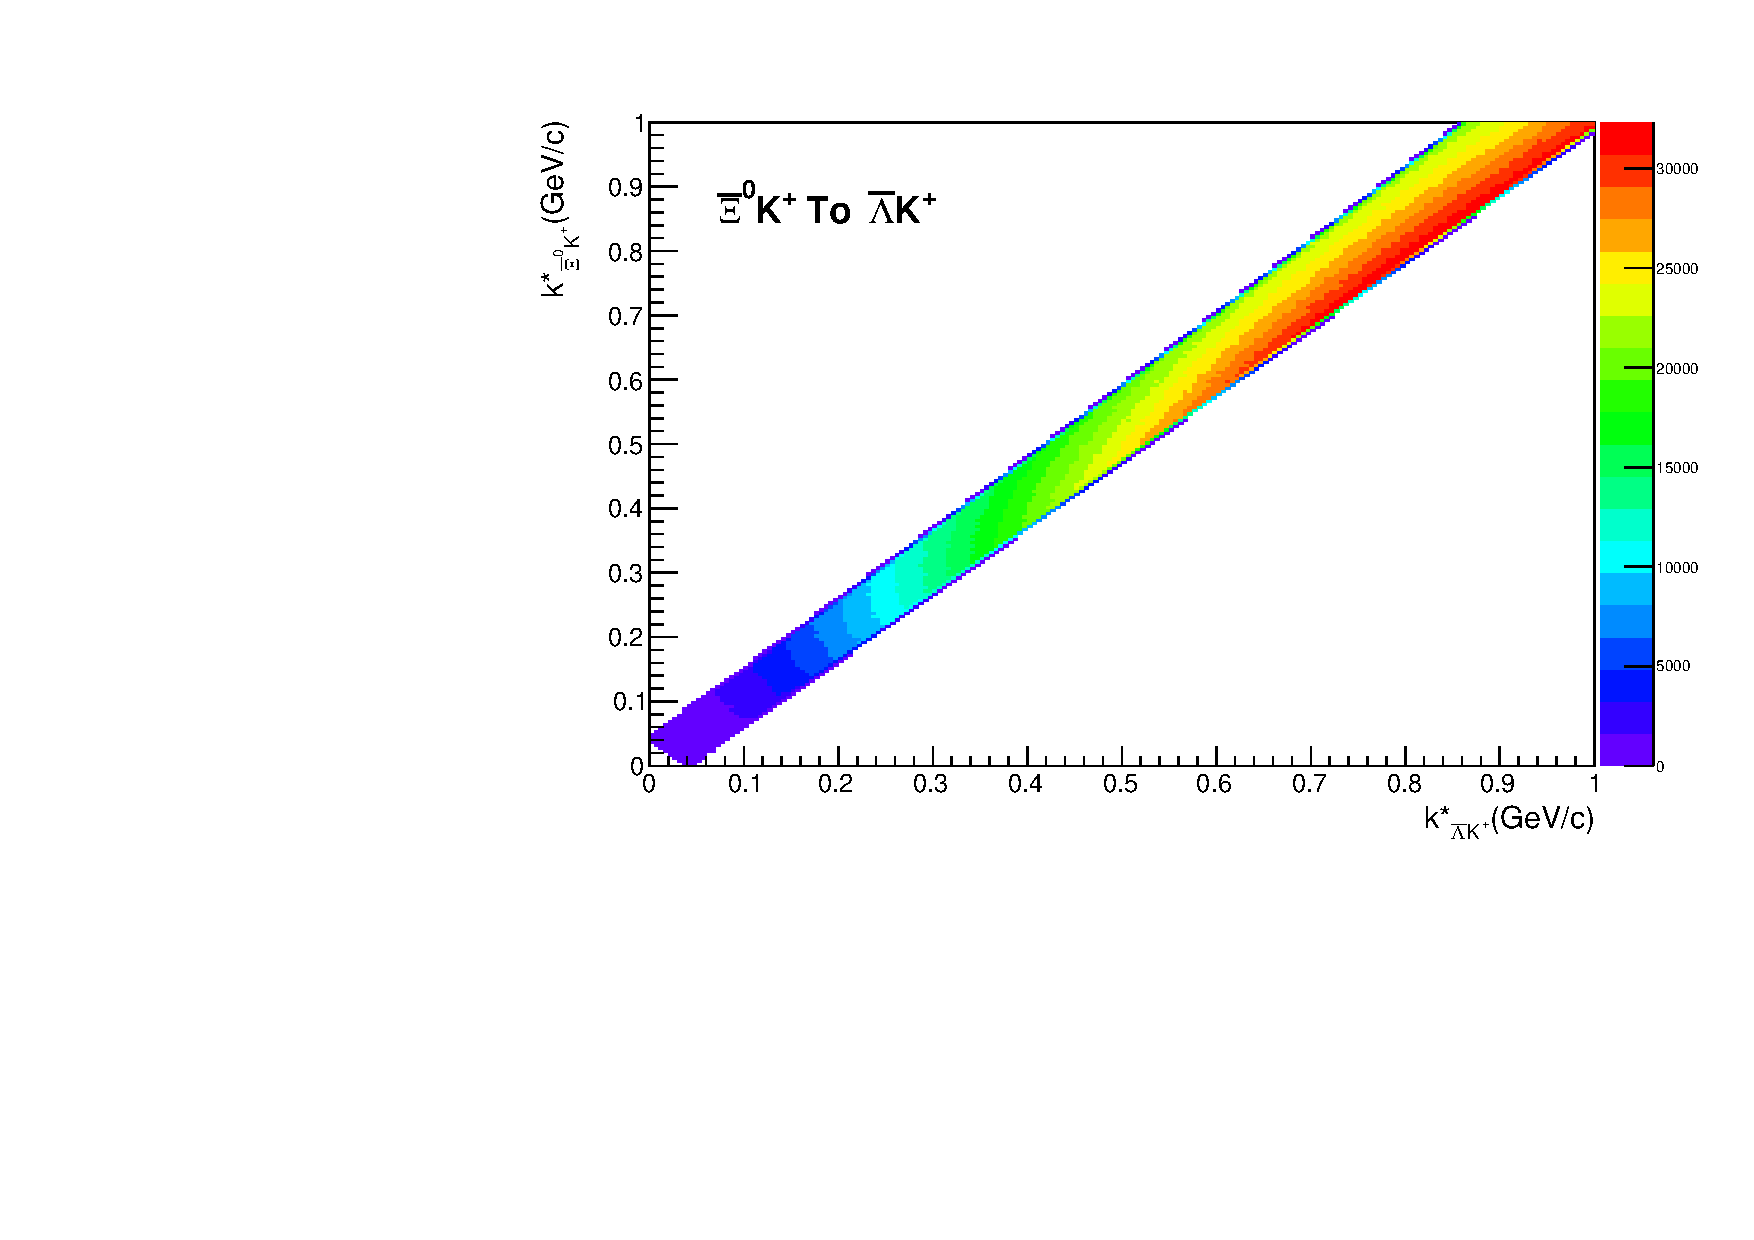
\includegraphics[width=0.49\textwidth]{5_Fitting/Figures/fAXi0ToALamKchPTransform.pdf}}
  %%----start of fourth subfigure---
  \subfloat[Transform matrix for $\bar{\Omega}^{+}$K$^{+}$ pairs into $\bar{\Lambda}$K$^{+}$]{
    \label{fig:TransformMatricesALamKchP:d}
    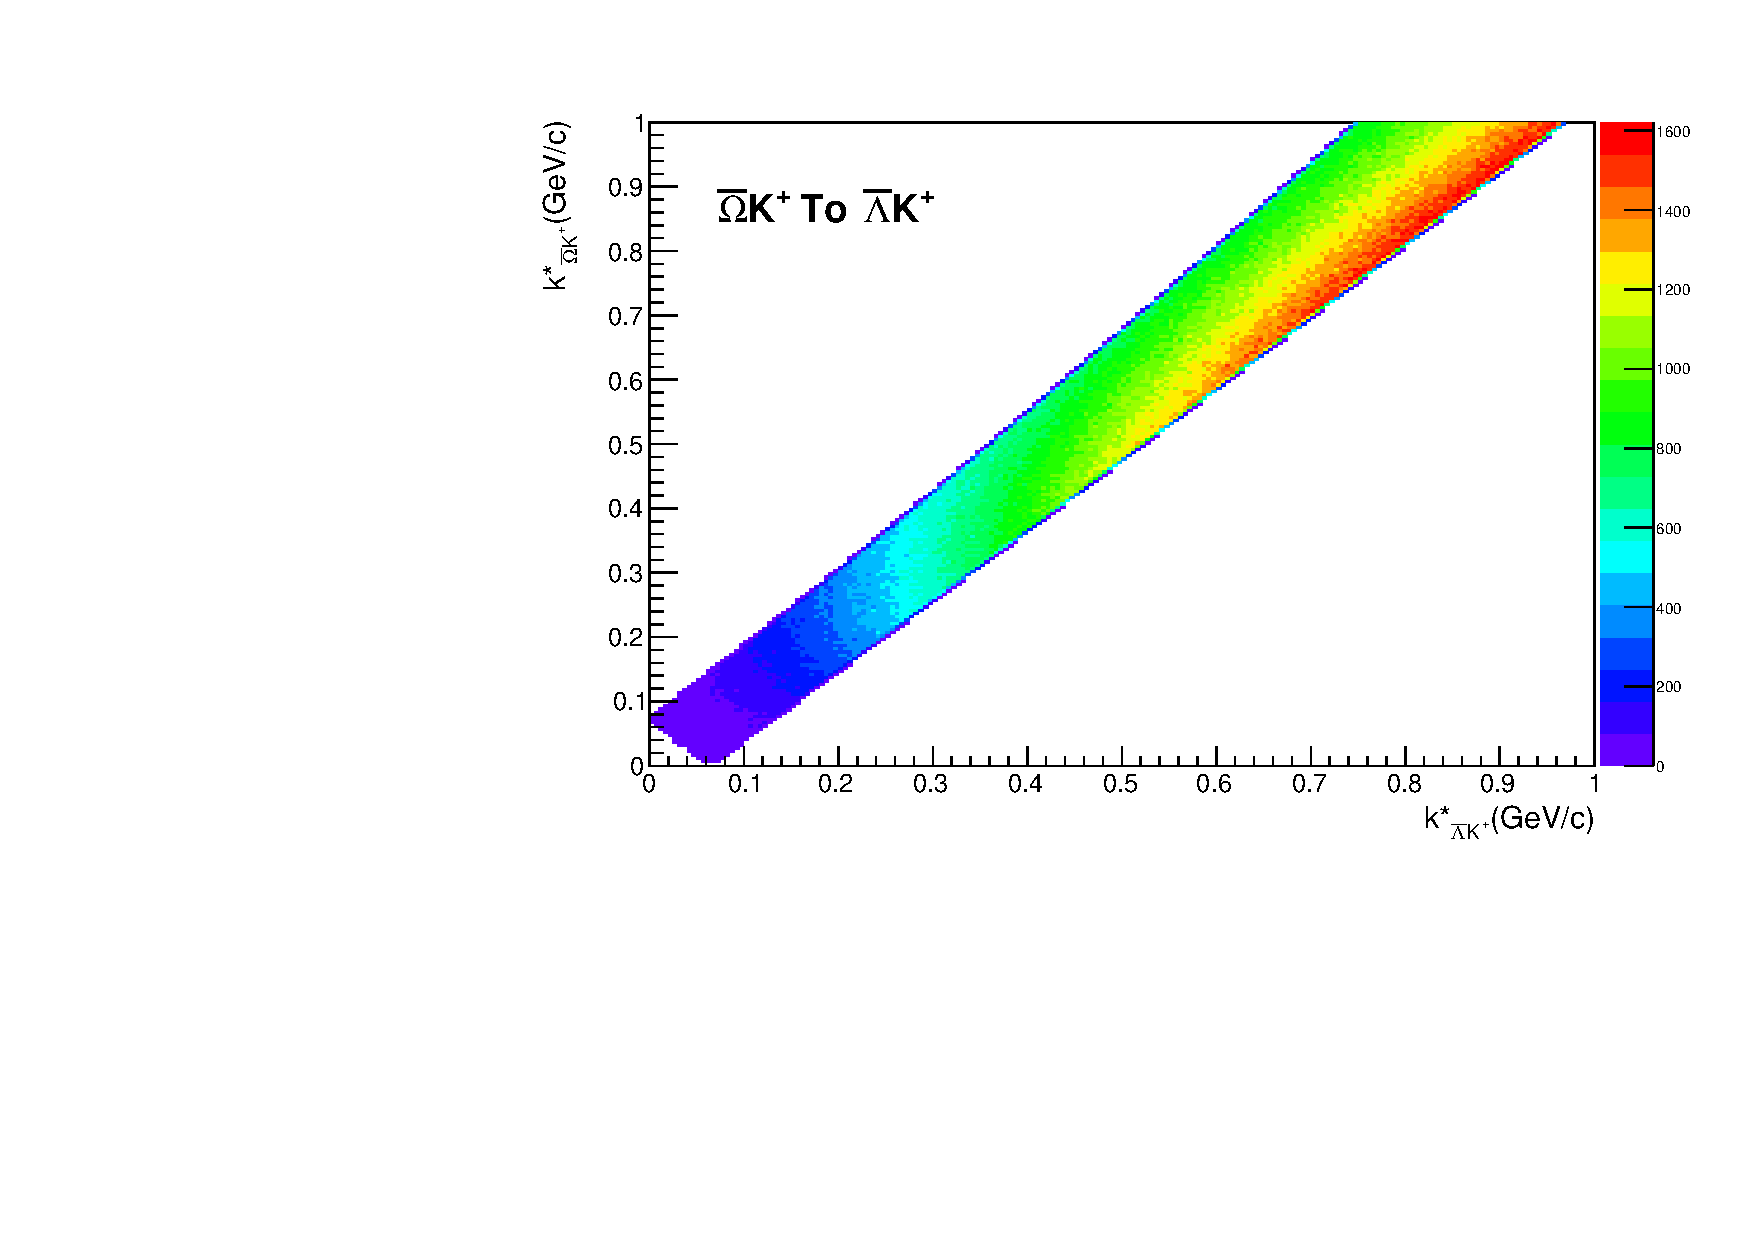
\includegraphics[width=0.49\textwidth]{5_Fitting/Figures/fAOmegaToALamKchPTransform.pdf}}                    
  %%----overall caption----
  \caption[Transform Matrices for $\bar{\Lambda}$K$^{+}$ Analysis]{Transform Matrices generated with THERMINATOR for $\bar{\Lambda}$K$^{+}$ Analysis}
  \label{fig:TransformMatricesALamKchP}
\end{figure}

\end{document}